\section{Supporting Multiple Names}

One of the goals of the naming scheme in StreamFS is to support multiple names for sensor and actuators.  The inclusion of symlinks 
provides this ability.  A file can be named and linked to from multiple hierarchies.  This allows applications to refer
to the same physical entity with a unique object id through multiple names.  It is also used by our pub-sub system when
the names are resolved and play a crucial role in \emph{dynamic aggregation}.

For example, a temperature sensor may have at least two names that are expose to the end user.  It may have a name that refers to 
it through the context of its spatial placement, such as \texttt{/soda/4F/410R/temp} and it may have a name that refers to it 
through the context of its association with a component in the HVAC system, such as \texttt{/soda/hvac/ahu1/vent1/temp}.  Either
of those are names that should access the same item and that item's associated data.  The underlying stream may actually write
the data to a stream file named \texttt{/strms/temp} and the other two names are just symlinks to this one.  

The pub-sub system uses these names when decided which data streams match a subscription topic.  For example, in a typical pub-sub system,
if a job wanted to subscribe to the temp stream, it would have to know the name \emph{a priori}, or simply pick a single name.
However, we support the notion of multi-topic stream tags.  So, if a subscriber request all the streams with the topic 
\texttt{/soda/4F/410R/*} and a data point is written to \texttt{/strm/temp}, the subscription manager would list all the aliases
for that name, which include \texttt{/soda/4F/410R/temp} and see that it matches the topic request for that subscription.

Notice how naming explicitly affects how we group sensors according to some hiearchical organization.  Some of those groupings
are physical associations with one another that are important to stay accurate.  Let's re-examine the example presented in
section~\ref{sec:cntxtacc}.  We present the figure from that section again in Figure~\ref{fig:mpc_example2}.

% walk through the example and show how multinaming helps address this and 
% why it's important to get right -- that should lead us right into the next section with no problem.

\begin{figure}[h!] %htbp
\centering
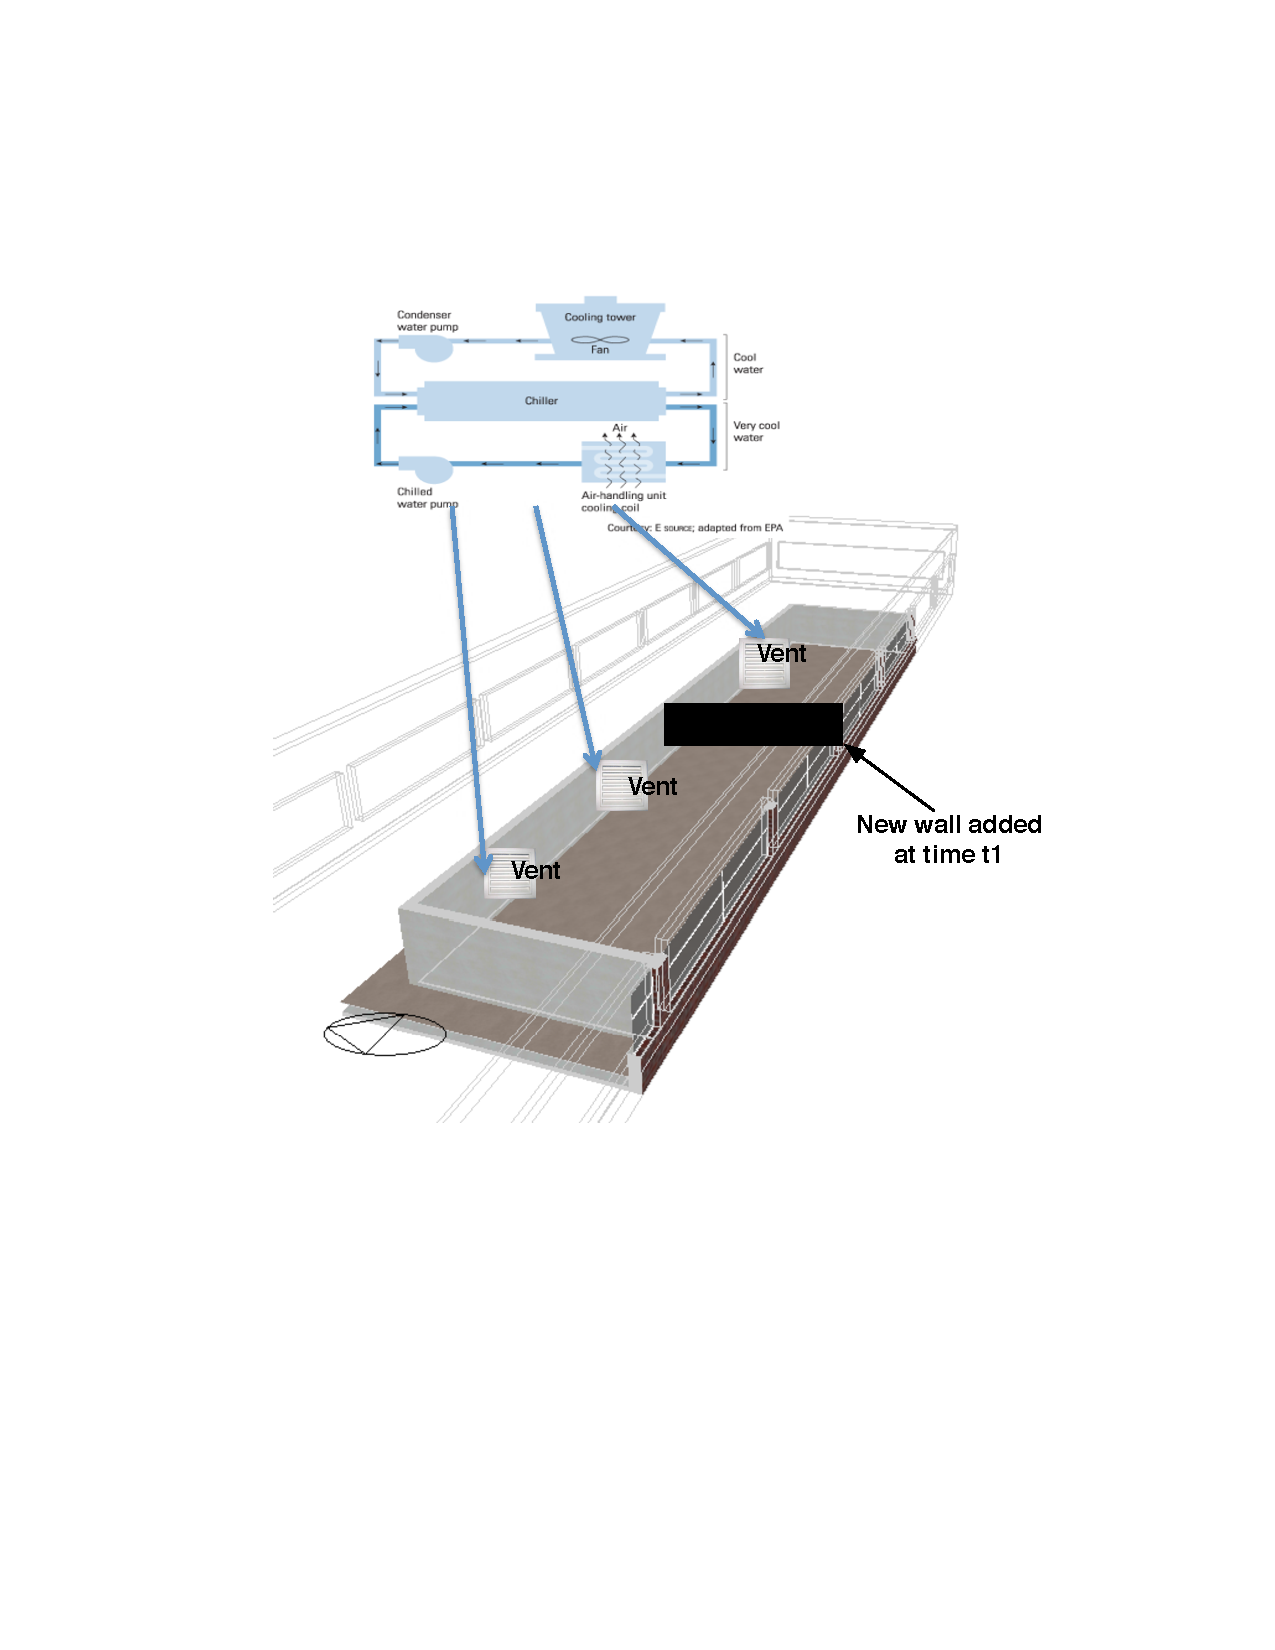
\includegraphics[width=0.5\columnwidth]{figs/mpc_example}
\caption{MPC example where metadata must be verified to maintain correct behavior.}
\label{fig:mpc_example2}
\end{figure}

Recall that the equation that drive the control process depending on knowing the mapping between vents and rooms.  Therefore,
if the room changes and a vent is added or removed, the control algorithm must be updated to account for the change.  The naming
structure would contain a reference to the vent in some group, linked to a sensor that belongs to a certain room, however,
if a wall is put up, we should be able to automatically detect that this has occurred to update the control process.
In summary, the naming scheme is used to express different kinds of organizational patterns for the sensors and their data.
As the building goes through some changes and evolves an automatic scheme or family of schemes are necessary to alert
the user or process of the chance.  In the next
section we discuss the mathematical tools we used to verify that the groups specified by the naming convention are correct.
